% Options for packages loaded elsewhere
\PassOptionsToPackage{unicode}{hyperref}
\PassOptionsToPackage{hyphens}{url}
\PassOptionsToPackage{dvipsnames,svgnames,x11names}{xcolor}
%
\documentclass[
  letterpaper,
  DIV=11,
  numbers=noendperiod]{scrartcl}

\usepackage{amsmath,amssymb}
\usepackage{iftex}
\ifPDFTeX
  \usepackage[T1]{fontenc}
  \usepackage[utf8]{inputenc}
  \usepackage{textcomp} % provide euro and other symbols
\else % if luatex or xetex
  \usepackage{unicode-math}
  \defaultfontfeatures{Scale=MatchLowercase}
  \defaultfontfeatures[\rmfamily]{Ligatures=TeX,Scale=1}
\fi
\usepackage{lmodern}
\ifPDFTeX\else  
    % xetex/luatex font selection
\fi
% Use upquote if available, for straight quotes in verbatim environments
\IfFileExists{upquote.sty}{\usepackage{upquote}}{}
\IfFileExists{microtype.sty}{% use microtype if available
  \usepackage[]{microtype}
  \UseMicrotypeSet[protrusion]{basicmath} % disable protrusion for tt fonts
}{}
\makeatletter
\@ifundefined{KOMAClassName}{% if non-KOMA class
  \IfFileExists{parskip.sty}{%
    \usepackage{parskip}
  }{% else
    \setlength{\parindent}{0pt}
    \setlength{\parskip}{6pt plus 2pt minus 1pt}}
}{% if KOMA class
  \KOMAoptions{parskip=half}}
\makeatother
\usepackage{xcolor}
\setlength{\emergencystretch}{3em} % prevent overfull lines
\setcounter{secnumdepth}{-\maxdimen} % remove section numbering
% Make \paragraph and \subparagraph free-standing
\makeatletter
\ifx\paragraph\undefined\else
  \let\oldparagraph\paragraph
  \renewcommand{\paragraph}{
    \@ifstar
      \xxxParagraphStar
      \xxxParagraphNoStar
  }
  \newcommand{\xxxParagraphStar}[1]{\oldparagraph*{#1}\mbox{}}
  \newcommand{\xxxParagraphNoStar}[1]{\oldparagraph{#1}\mbox{}}
\fi
\ifx\subparagraph\undefined\else
  \let\oldsubparagraph\subparagraph
  \renewcommand{\subparagraph}{
    \@ifstar
      \xxxSubParagraphStar
      \xxxSubParagraphNoStar
  }
  \newcommand{\xxxSubParagraphStar}[1]{\oldsubparagraph*{#1}\mbox{}}
  \newcommand{\xxxSubParagraphNoStar}[1]{\oldsubparagraph{#1}\mbox{}}
\fi
\makeatother

\usepackage{color}
\usepackage{fancyvrb}
\newcommand{\VerbBar}{|}
\newcommand{\VERB}{\Verb[commandchars=\\\{\}]}
\DefineVerbatimEnvironment{Highlighting}{Verbatim}{commandchars=\\\{\}}
% Add ',fontsize=\small' for more characters per line
\usepackage{framed}
\definecolor{shadecolor}{RGB}{241,243,245}
\newenvironment{Shaded}{\begin{snugshade}}{\end{snugshade}}
\newcommand{\AlertTok}[1]{\textcolor[rgb]{0.68,0.00,0.00}{#1}}
\newcommand{\AnnotationTok}[1]{\textcolor[rgb]{0.37,0.37,0.37}{#1}}
\newcommand{\AttributeTok}[1]{\textcolor[rgb]{0.40,0.45,0.13}{#1}}
\newcommand{\BaseNTok}[1]{\textcolor[rgb]{0.68,0.00,0.00}{#1}}
\newcommand{\BuiltInTok}[1]{\textcolor[rgb]{0.00,0.23,0.31}{#1}}
\newcommand{\CharTok}[1]{\textcolor[rgb]{0.13,0.47,0.30}{#1}}
\newcommand{\CommentTok}[1]{\textcolor[rgb]{0.37,0.37,0.37}{#1}}
\newcommand{\CommentVarTok}[1]{\textcolor[rgb]{0.37,0.37,0.37}{\textit{#1}}}
\newcommand{\ConstantTok}[1]{\textcolor[rgb]{0.56,0.35,0.01}{#1}}
\newcommand{\ControlFlowTok}[1]{\textcolor[rgb]{0.00,0.23,0.31}{\textbf{#1}}}
\newcommand{\DataTypeTok}[1]{\textcolor[rgb]{0.68,0.00,0.00}{#1}}
\newcommand{\DecValTok}[1]{\textcolor[rgb]{0.68,0.00,0.00}{#1}}
\newcommand{\DocumentationTok}[1]{\textcolor[rgb]{0.37,0.37,0.37}{\textit{#1}}}
\newcommand{\ErrorTok}[1]{\textcolor[rgb]{0.68,0.00,0.00}{#1}}
\newcommand{\ExtensionTok}[1]{\textcolor[rgb]{0.00,0.23,0.31}{#1}}
\newcommand{\FloatTok}[1]{\textcolor[rgb]{0.68,0.00,0.00}{#1}}
\newcommand{\FunctionTok}[1]{\textcolor[rgb]{0.28,0.35,0.67}{#1}}
\newcommand{\ImportTok}[1]{\textcolor[rgb]{0.00,0.46,0.62}{#1}}
\newcommand{\InformationTok}[1]{\textcolor[rgb]{0.37,0.37,0.37}{#1}}
\newcommand{\KeywordTok}[1]{\textcolor[rgb]{0.00,0.23,0.31}{\textbf{#1}}}
\newcommand{\NormalTok}[1]{\textcolor[rgb]{0.00,0.23,0.31}{#1}}
\newcommand{\OperatorTok}[1]{\textcolor[rgb]{0.37,0.37,0.37}{#1}}
\newcommand{\OtherTok}[1]{\textcolor[rgb]{0.00,0.23,0.31}{#1}}
\newcommand{\PreprocessorTok}[1]{\textcolor[rgb]{0.68,0.00,0.00}{#1}}
\newcommand{\RegionMarkerTok}[1]{\textcolor[rgb]{0.00,0.23,0.31}{#1}}
\newcommand{\SpecialCharTok}[1]{\textcolor[rgb]{0.37,0.37,0.37}{#1}}
\newcommand{\SpecialStringTok}[1]{\textcolor[rgb]{0.13,0.47,0.30}{#1}}
\newcommand{\StringTok}[1]{\textcolor[rgb]{0.13,0.47,0.30}{#1}}
\newcommand{\VariableTok}[1]{\textcolor[rgb]{0.07,0.07,0.07}{#1}}
\newcommand{\VerbatimStringTok}[1]{\textcolor[rgb]{0.13,0.47,0.30}{#1}}
\newcommand{\WarningTok}[1]{\textcolor[rgb]{0.37,0.37,0.37}{\textit{#1}}}

\providecommand{\tightlist}{%
  \setlength{\itemsep}{0pt}\setlength{\parskip}{0pt}}\usepackage{longtable,booktabs,array}
\usepackage{calc} % for calculating minipage widths
% Correct order of tables after \paragraph or \subparagraph
\usepackage{etoolbox}
\makeatletter
\patchcmd\longtable{\par}{\if@noskipsec\mbox{}\fi\par}{}{}
\makeatother
% Allow footnotes in longtable head/foot
\IfFileExists{footnotehyper.sty}{\usepackage{footnotehyper}}{\usepackage{footnote}}
\makesavenoteenv{longtable}
\usepackage{graphicx}
\makeatletter
\def\maxwidth{\ifdim\Gin@nat@width>\linewidth\linewidth\else\Gin@nat@width\fi}
\def\maxheight{\ifdim\Gin@nat@height>\textheight\textheight\else\Gin@nat@height\fi}
\makeatother
% Scale images if necessary, so that they will not overflow the page
% margins by default, and it is still possible to overwrite the defaults
% using explicit options in \includegraphics[width, height, ...]{}
\setkeys{Gin}{width=\maxwidth,height=\maxheight,keepaspectratio}
% Set default figure placement to htbp
\makeatletter
\def\fps@figure{htbp}
\makeatother

\KOMAoption{captions}{tableheading}
\makeatletter
\@ifpackageloaded{caption}{}{\usepackage{caption}}
\AtBeginDocument{%
\ifdefined\contentsname
  \renewcommand*\contentsname{Table of contents}
\else
  \newcommand\contentsname{Table of contents}
\fi
\ifdefined\listfigurename
  \renewcommand*\listfigurename{List of Figures}
\else
  \newcommand\listfigurename{List of Figures}
\fi
\ifdefined\listtablename
  \renewcommand*\listtablename{List of Tables}
\else
  \newcommand\listtablename{List of Tables}
\fi
\ifdefined\figurename
  \renewcommand*\figurename{Figure}
\else
  \newcommand\figurename{Figure}
\fi
\ifdefined\tablename
  \renewcommand*\tablename{Table}
\else
  \newcommand\tablename{Table}
\fi
}
\@ifpackageloaded{float}{}{\usepackage{float}}
\floatstyle{ruled}
\@ifundefined{c@chapter}{\newfloat{codelisting}{h}{lop}}{\newfloat{codelisting}{h}{lop}[chapter]}
\floatname{codelisting}{Listing}
\newcommand*\listoflistings{\listof{codelisting}{List of Listings}}
\makeatother
\makeatletter
\makeatother
\makeatletter
\@ifpackageloaded{caption}{}{\usepackage{caption}}
\@ifpackageloaded{subcaption}{}{\usepackage{subcaption}}
\makeatother

\ifLuaTeX
  \usepackage{selnolig}  % disable illegal ligatures
\fi
\usepackage{bookmark}

\IfFileExists{xurl.sty}{\usepackage{xurl}}{} % add URL line breaks if available
\urlstyle{same} % disable monospaced font for URLs
\hypersetup{
  pdftitle={important if running on Colab},
  colorlinks=true,
  linkcolor={blue},
  filecolor={Maroon},
  citecolor={Blue},
  urlcolor={Blue},
  pdfcreator={LaTeX via pandoc}}


\title{important if running on Colab}
\author{}
\date{}

\begin{document}
\maketitle


\begin{Shaded}
\begin{Highlighting}[]
\CommentTok{\#If the cv2 module is not found, run that:}
\CommentTok{\#!pip install opencv{-}python}
\end{Highlighting}
\end{Shaded}

switch under runtime the ``Change runtime type'' to a GPU support. This
will speed up you calculations immensely

\begin{Shaded}
\begin{Highlighting}[]
\ImportTok{import}\NormalTok{ sys,os}
\ImportTok{import}\NormalTok{ numpy }\ImportTok{as}\NormalTok{ np                     }\CommentTok{\#main package for scientific computing with Python.}
\ImportTok{import}\NormalTok{ pandas }\ImportTok{as}\NormalTok{ pd                    }\CommentTok{\#main data handling package}
\ImportTok{from}\NormalTok{ matplotlib }\ImportTok{import}\NormalTok{ image           }\CommentTok{\#plot graphs in Python.}
\ImportTok{import}\NormalTok{ matplotlib.pyplot }\ImportTok{as}\NormalTok{ plt        }\CommentTok{\#lazy plotting}
\ImportTok{import}\NormalTok{ cv2                             }\CommentTok{\#image opening}
\end{Highlighting}
\end{Shaded}

\section{Building and training a neural
network}\label{building-and-training-a-neural-network}

In this notebook, we are going to see and build the basic components of
neural networks. We will first build from scratch a two layer neural
network that we will then train to separate images from birds and images
from dogs. The we will use Torch with a similar network and finally use
Keras to build a sequential neural network with some advanced
corrections

There are six components to artificial neurons. From left (input) to
right (output). If we only consider numerical values these are:

\begin{enumerate}
\def\labelenumi{\arabic{enumi}.}
\tightlist
\item
  Input nodes. Each input node is a real number
\item
  Connections with weight. Each connection that departs from the input
  node has a weight, which is also a real number.
\item
  Calculate a weighted sum: \(y = \sum_{i=1}^{D} w_i*x_i\)
\item
  Feed this sum into a transfer or activation function. this can be
  idendity, but normally this is a treshold function.
  e.g.~\(\left\{\begin{matrix}
  =0 \;\text{if}\; x\leq 0.5\\
  =1 \;\text{if}\; x>0.5
  \end{matrix}\right.\) Which however is not smooth, so alternatively a
  continous (sigmoid) function such as the logistic function is an
  alternative (see below)
\item
  output node of this chain
\item
  A perceptron is sometimes added to this, often this is called a bias,
  Which is an input node with a fixed value
\end{enumerate}

With the percepton the treshold is easier defined, meaning that the
transfer function can be switching at zero. (sometimes called ReLU
Rectifying Linear Unit) There are other variants, but we will talk about
them in the Keras section.

\begin{Shaded}
\begin{Highlighting}[]
\NormalTok{x}\OperatorTok{=}\NormalTok{np.arange(}\OperatorTok{{-}}\DecValTok{10}\NormalTok{,}\DecValTok{10}\NormalTok{,}\FloatTok{0.1}\NormalTok{)}\OperatorTok{;}\NormalTok{y}\OperatorTok{=}\NormalTok{np.exp(x)}\OperatorTok{/}\NormalTok{(}\DecValTok{1} \OperatorTok{+}\NormalTok{ np.exp(x))}
\NormalTok{fig,ax}\OperatorTok{=}\NormalTok{plt.subplots()}\OperatorTok{;}\NormalTok{plt.plot(x,y)}\OperatorTok{;}\NormalTok{ax.set\_title(}\StringTok{\textquotesingle{}One logistic function\textquotesingle{}}\NormalTok{)}
\end{Highlighting}
\end{Shaded}

\begin{verbatim}
Text(0.5, 1.0, 'One logistic function')
\end{verbatim}

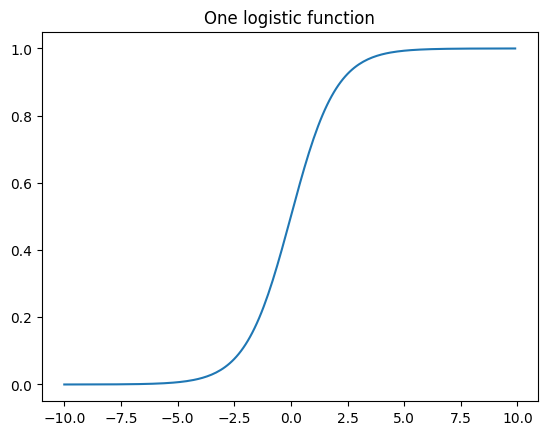
\includegraphics{NeuralNetworks_1_files/figure-pdf/cell-4-output-2.png}

\section{Data Loading}\label{data-loading}

Now, we load the data that we will need for the NN

\begin{Shaded}
\begin{Highlighting}[]
\ImportTok{import}\NormalTok{ sys}
\ControlFlowTok{if} \StringTok{"google.colab"} \KeywordTok{in}\NormalTok{ sys.modules:}
\NormalTok{    path\_to\_files }\OperatorTok{=}\NormalTok{ os.sep.join([os.getcwd(), }\StringTok{"Bern02"}\NormalTok{, }\StringTok{"Labs"}\NormalTok{, }\StringTok{"Neural\_Networks"}\NormalTok{, }\StringTok{"train"}\NormalTok{])}
    \OperatorTok{!}\NormalTok{git clone https:}\OperatorTok{//}\NormalTok{github.com}\OperatorTok{/}\NormalTok{luchem}\OperatorTok{/}\NormalTok{Bern02.git }\OperatorTok{{-}{-}}\NormalTok{depth}\OperatorTok{=}\DecValTok{1}
\ControlFlowTok{else}\NormalTok{:}
\NormalTok{    path\_to\_files }\OperatorTok{=}\NormalTok{ os.sep.join([os.getcwd(), }\StringTok{"train"}\NormalTok{])}
\end{Highlighting}
\end{Shaded}

\begin{Shaded}
\begin{Highlighting}[]
\CommentTok{\#We create two empty lists to store the data (the images) and the labels (0 if bird, 1 if dog)}
\NormalTok{data}\OperatorTok{=}\NormalTok{[]}
\NormalTok{labels}\OperatorTok{=}\NormalTok{[]}
\NormalTok{image\_size}\OperatorTok{=}\DecValTok{32}
\CommentTok{\#We now load the data into the notebook from the folder on your computer}
\ControlFlowTok{for}\NormalTok{ filename }\KeywordTok{in}\NormalTok{ os.listdir(os.sep.join([path\_to\_files,}\StringTok{\textquotesingle{}bird\textquotesingle{}}\NormalTok{])):}
\NormalTok{    labels.append(}\DecValTok{0}\NormalTok{)}
\NormalTok{    data.append(cv2.resize(image.imread(os.sep.join([path\_to\_files,}\StringTok{\textquotesingle{}bird\textquotesingle{}}\NormalTok{,filename])),dsize}\OperatorTok{=}\NormalTok{(image\_size,image\_size)))}
\ControlFlowTok{for}\NormalTok{ filename }\KeywordTok{in}\NormalTok{ os.listdir(os.sep.join([path\_to\_files,}\StringTok{\textquotesingle{}dog\textquotesingle{}}\NormalTok{])):}
\NormalTok{    labels.append(}\DecValTok{1}\NormalTok{)}
\NormalTok{    data.append(cv2.resize(image.imread(os.sep.join([path\_to\_files,}\StringTok{\textquotesingle{}dog\textquotesingle{}}\NormalTok{,filename])),dsize}\OperatorTok{=}\NormalTok{(image\_size,image\_size)))}
\NormalTok{data}\OperatorTok{=}\NormalTok{np.array(data)}
\NormalTok{labels}\OperatorTok{=}\NormalTok{np.array(labels)}
\end{Highlighting}
\end{Shaded}

\begin{verbatim}
FileNotFoundError: [Errno 2] No such file or directory: '/home/melanie/Documents/schoolstuff/Reprod_datascience/Labs/Lab9_NN/train/bird'
---------------------------------------------------------------------------
FileNotFoundError                         Traceback (most recent call last)
Cell In[5], line 6
      4 image_size=32
      5 #We now load the data into the notebook from the folder on your computer
----> 6 for filename in os.listdir(os.sep.join([path_to_files,'bird'])):
      7     labels.append(0)
      8     data.append(cv2.resize(image.imread(os.sep.join([path_to_files,'bird',filename])),dsize=(image_size,image_size)))

FileNotFoundError: [Errno 2] No such file or directory: '/home/melanie/Documents/schoolstuff/Reprod_datascience/Labs/Lab9_NN/train/bird'
\end{verbatim}

Questions: How many data files do we have in total?

Lets split this data into a training and testing dataset. While there
are specific selectors for this we simply use a permutation of the
index.

\begin{Shaded}
\begin{Highlighting}[]
\NormalTok{np.random.seed(}\DecValTok{0}\NormalTok{)}
\NormalTok{idx}\OperatorTok{=}\NormalTok{np.random.permutation(}\BuiltInTok{len}\NormalTok{(labels))}
\NormalTok{idx\_train}\OperatorTok{=}\NormalTok{idx[}\DecValTok{0}\NormalTok{:}\DecValTok{2000}\NormalTok{]}
\NormalTok{idx\_test}\OperatorTok{=}\NormalTok{idx[}\DecValTok{2001}\NormalTok{:}\DecValTok{2401}\NormalTok{]}
\NormalTok{train\_x}\OperatorTok{=}\NormalTok{data[idx\_train]}
\NormalTok{test\_x}\OperatorTok{=}\NormalTok{data[idx\_test]}
\NormalTok{train\_y}\OperatorTok{=}\NormalTok{labels[idx\_train].reshape(}\DecValTok{1}\NormalTok{,}\OperatorTok{{-}}\DecValTok{1}\NormalTok{)}
\NormalTok{test\_y}\OperatorTok{=}\NormalTok{labels[idx\_test].reshape(}\DecValTok{1}\NormalTok{,}\OperatorTok{{-}}\DecValTok{1}\NormalTok{)}
\end{Highlighting}
\end{Shaded}

What is the size of the images? Does the size matter?

\section{Data Inspection}\label{data-inspection}

\begin{Shaded}
\begin{Highlighting}[]
\BuiltInTok{print}\NormalTok{(}\StringTok{\textquotesingle{}the shape of the image is:\textquotesingle{}}\NormalTok{)}
\BuiltInTok{print}\NormalTok{(train\_x[}\DecValTok{0}\NormalTok{].shape)}
\NormalTok{plt.imshow(train\_x[}\DecValTok{4}\NormalTok{])}
\end{Highlighting}
\end{Shaded}

\section{Data shaping}\label{data-shaping}

To avoid some divergence, we normalize the intensity of each pixels and
flatten it. The flattening is a simplification to not have to deal with
the dimensions. As we will be connecting every pixel the actual
positions do not matter. This will be different for convolutional
networks.

\begin{Shaded}
\begin{Highlighting}[]
\CommentTok{\# we use a single dimension layer, so flattening the matrix}
\NormalTok{train\_x\_flatten}\OperatorTok{=}\NormalTok{train\_x.reshape(train\_x.shape[}\DecValTok{0}\NormalTok{],}\OperatorTok{{-}}\DecValTok{1}\NormalTok{).T}
\NormalTok{test\_x\_flatten}\OperatorTok{=}\NormalTok{test\_x.reshape(test\_x.shape[}\DecValTok{0}\NormalTok{],}\OperatorTok{{-}}\DecValTok{1}\NormalTok{).T}
\CommentTok{\# all values must be "normalized" meaning between 0 and 1}
\NormalTok{train\_x\_flatten}\OperatorTok{=}\NormalTok{train\_x\_flatten}\OperatorTok{/}\DecValTok{255}
\NormalTok{test\_x\_flatten}\OperatorTok{=}\NormalTok{test\_x\_flatten}\OperatorTok{/}\DecValTok{255}
\end{Highlighting}
\end{Shaded}

We will build a neural network with 2 layers First we start by building
the neural net. For this we we initialize the weights and biases for
each layer.

\section{Neuronal net building}\label{neuronal-net-building}

\begin{Shaded}
\begin{Highlighting}[]
\KeywordTok{def}\NormalTok{ initialize\_parameters(n\_x, n\_h, n\_y):}
    \CommentTok{"""}
\CommentTok{    n\_x {-}{-} size of input layer; }
\CommentTok{    n\_h {-}{-} size of hidden layer; }
\CommentTok{    n\_y {-}{-} size of output layer}
\CommentTok{    Returns:}
\CommentTok{    parameters {-}{-} python dictionary containing your parameters:             }
\CommentTok{    """}
\NormalTok{    W1 }\OperatorTok{=}\NormalTok{ np.random.randn(n\_h, n\_x) }\OperatorTok{*} \FloatTok{0.01} \CommentTok{\#W1 {-}{-} weight matrix of shape (n\_h, n\_x)}
\NormalTok{    b1 }\OperatorTok{=}\NormalTok{ np.zeros((n\_h, }\DecValTok{1}\NormalTok{))               }\CommentTok{\#b1 {-}{-} bias vector of shape (n\_h, 1)}
\NormalTok{    W2 }\OperatorTok{=}\NormalTok{ np.random.randn(n\_y, n\_h) }\OperatorTok{*} \FloatTok{0.01} \CommentTok{\#W2 {-}{-} weight matrix of shape (n\_y, n\_h)}
\NormalTok{    b2 }\OperatorTok{=}\NormalTok{ np.zeros((n\_y, }\DecValTok{1}\NormalTok{))               }\CommentTok{\#b2 {-}{-} bias vector of shape (n\_y, 1)    }
\NormalTok{    parameters }\OperatorTok{=}\NormalTok{ \{}\StringTok{"W1"}\NormalTok{: W1,}
                  \StringTok{"b1"}\NormalTok{: b1,}
                  \StringTok{"W2"}\NormalTok{: W2,}
                  \StringTok{"b2"}\NormalTok{: b2\}}
    \ControlFlowTok{return}\NormalTok{ parameters}
\end{Highlighting}
\end{Shaded}

We now code the forward propagation through (from the input to the
output (left to right)

\begin{Shaded}
\begin{Highlighting}[]
\KeywordTok{def}\NormalTok{ linear\_forward(Input\_Matrix, Weights, bias):}
    \CommentTok{"""}
\CommentTok{    function to calculate the combination of Input, weights and bias}
\CommentTok{    forward propagation.}
\CommentTok{    Returns: Output\_Matrix, (Input\_Matrix, Weights, bias)}
\CommentTok{    """}
\NormalTok{    Output\_Matrix }\OperatorTok{=}\NormalTok{ np.dot(Weights, Input\_Matrix) }\OperatorTok{+}\NormalTok{ bias}
\NormalTok{    cache }\OperatorTok{=}\NormalTok{ (Input\_Matrix, Weights, bias)}
    \ControlFlowTok{return}\NormalTok{ Output\_Matrix, cache}
\KeywordTok{def}\NormalTok{ relu(Z):}\CommentTok{\# forward activation (rectification function)}
    \ControlFlowTok{return}\NormalTok{ np.maximum(np.zeros(Z.shape),Z),Z}
\KeywordTok{def}\NormalTok{ sigmoid(Z): }\CommentTok{\# forward activation (smooth rectification)}
    \ControlFlowTok{return} \DecValTok{1}\OperatorTok{/}\NormalTok{(}\DecValTok{1}\OperatorTok{+}\NormalTok{np.exp(}\OperatorTok{{-}}\NormalTok{Z)),Z}
\KeywordTok{def}\NormalTok{ linear\_activation\_forward(Input\_Matrix, Weights, bias, activation\_method):}
    \CommentTok{"""}
\CommentTok{    Input\_Matrix: size of previous layer}
\CommentTok{    Weights: numpy array of shape (size of current layer, size of previous layer)}
\CommentTok{    bias vector, numpy array of shape (size of the current layer, 1)}
\CommentTok{    activation {-}{-} the activation to be used in this layer "sigmoid" or "relu"}
\CommentTok{    Returns: Output\_Matrix, (linear\_cache, activation\_cache)}
\CommentTok{    """}
    \ControlFlowTok{if}\NormalTok{ activation\_method }\OperatorTok{==} \StringTok{"sigmoid"}\NormalTok{:}
\NormalTok{        Z, linear\_cache }\OperatorTok{=}\NormalTok{ linear\_forward(Input\_Matrix, Weights, bias)}
\NormalTok{        Output\_Matrix, activation\_cache }\OperatorTok{=}\NormalTok{ sigmoid(Z)    }
    \ControlFlowTok{elif}\NormalTok{ activation\_method }\OperatorTok{==} \StringTok{"relu"}\NormalTok{:}
\NormalTok{        Z, linear\_cache }\OperatorTok{=}\NormalTok{ linear\_forward(Input\_Matrix, Weights, bias)}
\NormalTok{        Output\_Matrix, activation\_cache }\OperatorTok{=}\NormalTok{ relu(Z)    }
\NormalTok{    cache }\OperatorTok{=}\NormalTok{ (linear\_cache, activation\_cache)}
    \ControlFlowTok{return}\NormalTok{ Output\_Matrix, cache}
\end{Highlighting}
\end{Shaded}

\begin{Shaded}
\begin{Highlighting}[]
\KeywordTok{def}\NormalTok{ compute\_cost(Calculated\_classiciation,True\_classification):}
    \CommentTok{"""Calculate the cost=error of the current prediction"""}
\NormalTok{    m }\OperatorTok{=}\NormalTok{ True\_classification.shape[}\DecValTok{1}\NormalTok{] }\CommentTok{\#get size of vector}
\NormalTok{    a}\OperatorTok{=}\NormalTok{np.multiply(np.log(Calculated\_classiciation),True\_classification)}
\NormalTok{    b}\OperatorTok{=}\NormalTok{np.multiply(np.log(}\DecValTok{1}\OperatorTok{{-}}\NormalTok{Calculated\_classiciation),}\DecValTok{1}\OperatorTok{{-}}\NormalTok{True\_classification)}
\NormalTok{    cost }\OperatorTok{=}\NormalTok{  (}\OperatorTok{{-}}\FloatTok{1.}\OperatorTok{/}\NormalTok{m)}\OperatorTok{*}\NormalTok{np.}\BuiltInTok{sum}\NormalTok{(a}\OperatorTok{+}\NormalTok{b)}
\NormalTok{    cost }\OperatorTok{=}\NormalTok{ np.squeeze(cost)}\CommentTok{\# To make sure your cost\textquotesingle{}s shape is what we expect (e.g. this turns [[17]] into 17).}
    \ControlFlowTok{return}\NormalTok{ cost}
\end{Highlighting}
\end{Shaded}

\begin{enumerate}
\def\labelenumi{\arabic{enumi}.}
\tightlist
\item
  In the forward propagate stage, the data flows through the network to
  get the outputs.
\item
  Then we use the loss function to calculate the total error.
\item
  Then we use a backward propagation algorithm to calculate the gradient
  of the loss function with respect to each weight and bias (without
  having to actualy calculate differentials = more efficient) This
  gradient helps us to predict how we should adjust the parameter of the
  weights more efficiently
\end{enumerate}

\begin{Shaded}
\begin{Highlighting}[]
\KeywordTok{def}\NormalTok{ linear\_backward(dCost, cache):}
    \CommentTok{"""linear backward step}
\CommentTok{    dCost=cost gradient, cache {-}{-} from forward step (Input\_Matrix, Weights, bias) }
\CommentTok{    }
\CommentTok{    Returns:}
\CommentTok{    dInput {-}{-} Gradient of the cost with respect to the activation}
\CommentTok{    dW {-}{-} Gradient of the cost with respect to W (current layer l), same shape as W}
\CommentTok{    db {-}{-} Gradient of the cost with respect to b (current layer l), same shape as b}
\CommentTok{    """}
\NormalTok{    Input\_Matrix, Weights, bias }\OperatorTok{=}\NormalTok{ cache}
\NormalTok{    m }\OperatorTok{=}\NormalTok{ Input\_Matrix.shape[}\DecValTok{1}\NormalTok{]}
\NormalTok{    dWeights }\OperatorTok{=}\NormalTok{ (}\FloatTok{1.}\OperatorTok{/}\NormalTok{m)}\OperatorTok{*}\NormalTok{np.dot(dCost, Input\_Matrix.T)}
\NormalTok{    dbias }\OperatorTok{=}\NormalTok{ (}\FloatTok{1.}\OperatorTok{/}\NormalTok{m)}\OperatorTok{*}\NormalTok{np.}\BuiltInTok{sum}\NormalTok{(dCost, axis}\OperatorTok{=}\DecValTok{1}\NormalTok{, keepdims}\OperatorTok{=}\VariableTok{True}\NormalTok{)}
\NormalTok{    dActivation }\OperatorTok{=}\NormalTok{ np.dot(Weights.T, dCost)}
    \ControlFlowTok{return}\NormalTok{ dActivation, dWeights, dbias}

\KeywordTok{def}\NormalTok{ relu\_backward(dA, activation\_cache):}
    \ControlFlowTok{return}\NormalTok{ np.multiply(dA,np.heaviside(activation\_cache,}\DecValTok{0}\NormalTok{))}
\KeywordTok{def}\NormalTok{ sigmoid\_backward(dA,activation\_cache):}
    \ControlFlowTok{return}\NormalTok{ np.multiply(dA,np.multiply(sigmoid(activation\_cache)[}\DecValTok{0}\NormalTok{],np.ones(activation\_cache.shape)}\OperatorTok{{-}}\NormalTok{sigmoid(activation\_cache)[}\DecValTok{0}\NormalTok{]))}

\KeywordTok{def}\NormalTok{ linear\_activation\_backward(dCost, cache, activation\_method):}
    \CommentTok{"""Complete backward step:}
\CommentTok{    dCost {-}{-} cost gradient; }
\CommentTok{    cache {-}{-} (linear\_cache, activation\_cache); }
\CommentTok{    activation {-}{-} the method as string: "sigmoid" or "relu"}
\CommentTok{    }
\CommentTok{    Returns:}
\CommentTok{    dActivation, dCost in respect to activation}
\CommentTok{    dWeights, dCost in respect to weights}
\CommentTok{    dbias, dCost in respect to bias}
\CommentTok{    """}
\NormalTok{    linear\_cache, activation\_cache }\OperatorTok{=}\NormalTok{ cache}
    
    \ControlFlowTok{if}\NormalTok{ activation\_method }\OperatorTok{==} \StringTok{"relu"}\NormalTok{:}
\NormalTok{        dZ }\OperatorTok{=}\NormalTok{ relu\_backward(dCost, activation\_cache)}
\NormalTok{        dActivation, dWeights, dbias }\OperatorTok{=}\NormalTok{ linear\_backward(dZ, linear\_cache)}
    \ControlFlowTok{elif}\NormalTok{ activation\_method }\OperatorTok{==} \StringTok{"sigmoid"}\NormalTok{:}
\NormalTok{        dZ }\OperatorTok{=}\NormalTok{ sigmoid\_backward(dCost, activation\_cache)}
\NormalTok{        dActivation, dWeights, dbias }\OperatorTok{=}\NormalTok{ linear\_backward(dZ, linear\_cache)}
    \ControlFlowTok{return}\NormalTok{ dActivation, dWeights, dbias}
\end{Highlighting}
\end{Shaded}

\begin{Shaded}
\begin{Highlighting}[]
\KeywordTok{def}\NormalTok{ update\_parameters(parameters, gradients, learning\_rate):}
    \CommentTok{""" Update parameters using gradient descent}
\CommentTok{    Arguments: parameters (dict), gradients (dict), learning\_rate = L\_model\_backward}
\CommentTok{    Returns:}
\CommentTok{    updated parameters (dict)}
\CommentTok{    """}
\NormalTok{    L }\OperatorTok{=} \BuiltInTok{int}\NormalTok{(}\BuiltInTok{len}\NormalTok{(parameters.keys())}\OperatorTok{/}\DecValTok{2}\NormalTok{) }\CommentTok{\# number of layers in the neural network}
    \ControlFlowTok{for}\NormalTok{ l }\KeywordTok{in} \BuiltInTok{range}\NormalTok{(L):}
\NormalTok{        parameters[}\StringTok{"W}\SpecialCharTok{\%i}\StringTok{"}\OperatorTok{\%}\NormalTok{(l}\OperatorTok{+}\DecValTok{1}\NormalTok{)] }\OperatorTok{{-}=}\NormalTok{ learning\_rate }\OperatorTok{*}\NormalTok{ gradients[}\StringTok{"dW}\SpecialCharTok{\%i}\StringTok{"}\OperatorTok{\%}\NormalTok{(l}\OperatorTok{+}\DecValTok{1}\NormalTok{)]}
\NormalTok{        parameters[}\StringTok{"b}\SpecialCharTok{\%i}\StringTok{"}\OperatorTok{\%}\NormalTok{(l}\OperatorTok{+}\DecValTok{1}\NormalTok{)] }\OperatorTok{{-}=}\NormalTok{ learning\_rate }\OperatorTok{*}\NormalTok{ gradients[}\StringTok{"db}\SpecialCharTok{\%i}\StringTok{"}\OperatorTok{\%}\NormalTok{(l}\OperatorTok{+}\DecValTok{1}\NormalTok{)]  }
    \ControlFlowTok{return}\NormalTok{ parameters}
\end{Highlighting}
\end{Shaded}

\begin{Shaded}
\begin{Highlighting}[]
\KeywordTok{def}\NormalTok{ predictions(X,Y,parameters):}
    \CommentTok{\# Get W1, b1, W2 and b2 from the dictionary parameters.}
\NormalTok{    W1 }\OperatorTok{=}\NormalTok{ parameters[}\StringTok{"W1"}\NormalTok{]}
\NormalTok{    b1 }\OperatorTok{=}\NormalTok{ parameters[}\StringTok{"b1"}\NormalTok{]}
\NormalTok{    W2 }\OperatorTok{=}\NormalTok{ parameters[}\StringTok{"W2"}\NormalTok{]}
\NormalTok{    b2 }\OperatorTok{=}\NormalTok{ parameters[}\StringTok{"b2"}\NormalTok{]}
\NormalTok{    A1, cache1 }\OperatorTok{=}\NormalTok{ linear\_activation\_forward(X, W1, b1, activation\_method}\OperatorTok{=}\StringTok{\textquotesingle{}relu\textquotesingle{}}\NormalTok{)}
\NormalTok{    A2, cache2 }\OperatorTok{=}\NormalTok{ linear\_activation\_forward(A1, W2, b2, activation\_method}\OperatorTok{=}\StringTok{\textquotesingle{}sigmoid\textquotesingle{}}\NormalTok{)}
\NormalTok{    Z}\OperatorTok{=}\NormalTok{np.floor(A2}\OperatorTok{+}\FloatTok{0.5}\NormalTok{).astype(}\BuiltInTok{int}\NormalTok{)}
    \ControlFlowTok{return}\NormalTok{ np.}\BuiltInTok{sum}\NormalTok{((Z}\OperatorTok{==}\NormalTok{Y).astype(}\BuiltInTok{int}\NormalTok{))}\OperatorTok{/}\BuiltInTok{len}\NormalTok{(Y.T)}
\end{Highlighting}
\end{Shaded}

\begin{Shaded}
\begin{Highlighting}[]
\CommentTok{\#\#\# CONSTANTS DEFINING THE MODEL \#\#\#\#}
\NormalTok{n\_x }\OperatorTok{=}\NormalTok{ image\_size}\OperatorTok{*}\NormalTok{image\_size}\OperatorTok{*}\DecValTok{3}\CommentTok{\#3072     \# num\_px * num\_px * 3}
\NormalTok{n\_h }\OperatorTok{=} \DecValTok{128}  \CommentTok{\#we use these number nodes}
\NormalTok{n\_y }\OperatorTok{=} \DecValTok{1} \CommentTok{\#layer thickness}
\NormalTok{layers\_dims }\OperatorTok{=}\NormalTok{ (n\_x, n\_h, n\_y)}
\end{Highlighting}
\end{Shaded}

\begin{Shaded}
\begin{Highlighting}[]
\KeywordTok{def}\NormalTok{ two\_layer\_model(X, Y, layers\_dims, learning\_rate }\OperatorTok{=} \FloatTok{0.05}\NormalTok{, num\_iterations }\OperatorTok{=} \DecValTok{500}\NormalTok{, print\_cost\_every}\OperatorTok{=}\VariableTok{None}\NormalTok{):}
    \CommentTok{"""LINEAR{-}\textgreater{}RELU{-}\textgreater{}LINEAR{-}\textgreater{}SIGMOID.}
\CommentTok{    X Image\_input of shape (n\_x, number of examples)}
\CommentTok{    Y Vector with true "labels" (containing 0 if bird, 1 if dog)}
\CommentTok{    layers\_dims {-}{-} dimensions of the layers (n\_x, n\_h, n\_y)}
\CommentTok{    num\_iterations {-}{-} number of iterations of the optimization loop}
\CommentTok{    learning\_rate {-}{-} learning rate of the gradient descent update rule}
\CommentTok{    print\_cost\_every {-}{-} printing iteration}
\CommentTok{    Returns:}
\CommentTok{    parameters {-}{-} a dictionary containing W1, W2, b1, and b2}
\CommentTok{    """}
\NormalTok{    grads }\OperatorTok{=}\NormalTok{ \{\}}
\NormalTok{    costs }\OperatorTok{=}\NormalTok{ []                              }\CommentTok{\# to keep track of the cost}
\NormalTok{    m }\OperatorTok{=}\NormalTok{ X.shape[}\DecValTok{1}\NormalTok{]                           }\CommentTok{\# number of examples}
\NormalTok{    accuracy\_train}\OperatorTok{=}\NormalTok{[]}
\NormalTok{    accuracy\_test}\OperatorTok{=}\NormalTok{[]}
\NormalTok{    (n\_x, n\_h, n\_y) }\OperatorTok{=}\NormalTok{ layers\_dims}
    \CommentTok{\# Initialize parameters dictionary, by calling one of the functions you\textquotesingle{}d previously implemented}
\NormalTok{    parameters }\OperatorTok{=}\NormalTok{ initialize\_parameters(n\_x, n\_h, n\_y)}
    
    \ControlFlowTok{for}\NormalTok{ i }\KeywordTok{in} \BuiltInTok{range}\NormalTok{(}\DecValTok{0}\NormalTok{, num\_iterations):}\CommentTok{\# Loop (gradient descent)}
        
        \CommentTok{\# Forward propagation: LINEAR {-}\textgreater{} RELU {-}\textgreater{} LINEAR {-}\textgreater{} SIGMOID.}
\NormalTok{        A1, cache1 }\OperatorTok{=}\NormalTok{ linear\_activation\_forward(X, parameters[}\StringTok{"W1"}\NormalTok{], parameters[}\StringTok{"b1"}\NormalTok{], activation\_method}\OperatorTok{=}\StringTok{\textquotesingle{}relu\textquotesingle{}}\NormalTok{)}
\NormalTok{        A2, cache2 }\OperatorTok{=}\NormalTok{ linear\_activation\_forward(A1, parameters[}\StringTok{"W2"}\NormalTok{], parameters[}\StringTok{"b2"}\NormalTok{], activation\_method}\OperatorTok{=}\StringTok{\textquotesingle{}sigmoid\textquotesingle{}}\NormalTok{)}
        \CommentTok{\# Compute cost}
\NormalTok{        cost }\OperatorTok{=}\NormalTok{ compute\_cost(A2, Y)}
        \CommentTok{\# Initializing backward propagation}
\NormalTok{        dA2 }\OperatorTok{=} \OperatorTok{{-}}\NormalTok{ (np.divide(Y, A2) }\OperatorTok{{-}}\NormalTok{ np.divide(}\DecValTok{1} \OperatorTok{{-}}\NormalTok{ Y, }\DecValTok{1} \OperatorTok{{-}}\NormalTok{ A2))}
        \CommentTok{\# Backward propagation. (calculate gradients)}
\NormalTok{        dA1, dW2, db2 }\OperatorTok{=}\NormalTok{ linear\_activation\_backward(dA2, cache2, activation\_method}\OperatorTok{=}\StringTok{"sigmoid"}\NormalTok{)}
\NormalTok{        dA0, dW1, db1 }\OperatorTok{=}\NormalTok{ linear\_activation\_backward(dA1, cache1, activation\_method}\OperatorTok{=}\StringTok{"relu"}\NormalTok{)}
        \CommentTok{\# Set grads[\textquotesingle{}dWl\textquotesingle{}] to dW1, grads[\textquotesingle{}db1\textquotesingle{}] to db1, grads[\textquotesingle{}dW2\textquotesingle{}] to dW2, grads[\textquotesingle{}db2\textquotesingle{}] to db2}
\NormalTok{        grads[}\StringTok{\textquotesingle{}dW1\textquotesingle{}}\NormalTok{] }\OperatorTok{=}\NormalTok{ dW1}
\NormalTok{        grads[}\StringTok{\textquotesingle{}db1\textquotesingle{}}\NormalTok{] }\OperatorTok{=}\NormalTok{ db1}
\NormalTok{        grads[}\StringTok{\textquotesingle{}dW2\textquotesingle{}}\NormalTok{] }\OperatorTok{=}\NormalTok{ dW2}
\NormalTok{        grads[}\StringTok{\textquotesingle{}db2\textquotesingle{}}\NormalTok{] }\OperatorTok{=}\NormalTok{ db2}
        
        \CommentTok{\# Update parameters.}
\NormalTok{        learning\_rate}\OperatorTok{*=}\FloatTok{0.999}
\NormalTok{        parameters }\OperatorTok{=}\NormalTok{ update\_parameters(parameters, grads, learning\_rate)}
        \CommentTok{\# Print the cost every 20 training example}
        \ControlFlowTok{if}\NormalTok{ print\_cost\_every }\KeywordTok{is} \VariableTok{None}\NormalTok{:}
            \ControlFlowTok{continue}
        \ControlFlowTok{else}\NormalTok{:}
            \ControlFlowTok{if}\NormalTok{ i }\OperatorTok{\%}\NormalTok{ print\_cost\_every }\OperatorTok{==} \DecValTok{0}\NormalTok{:}
\NormalTok{                accur}\OperatorTok{=}\NormalTok{predictions(train\_x\_flatten,train\_y,parameters)}
\NormalTok{                accur2}\OperatorTok{=}\NormalTok{predictions(test\_x\_flatten,test\_y,parameters)}
\NormalTok{                accuracy\_train.append(accur)}
\NormalTok{                accuracy\_test.append(accur2)}
\NormalTok{                costs.append(cost)}
                \BuiltInTok{print}\NormalTok{(}\StringTok{"Train accuracy after iteration }\SpecialCharTok{\{\}}\StringTok{: }\SpecialCharTok{\{\}}\StringTok{"}\NormalTok{.}\BuiltInTok{format}\NormalTok{(i,accur))}
                \BuiltInTok{print}\NormalTok{(}\StringTok{"Test accuracy after iteration }\SpecialCharTok{\{\}}\StringTok{: }\SpecialCharTok{\{\}}\StringTok{"}\NormalTok{.}\BuiltInTok{format}\NormalTok{(i,accur2))}
\NormalTok{    accur}\OperatorTok{=}\NormalTok{predictions(train\_x\_flatten,train\_y,parameters)}
\NormalTok{    accur2}\OperatorTok{=}\NormalTok{predictions(test\_x\_flatten,test\_y,parameters)}
\NormalTok{    accuracy\_train.append(accur)}
\NormalTok{    accuracy\_test.append(accur2)}
\NormalTok{    costs.append(cost)}
    \ControlFlowTok{if}\NormalTok{ print\_cost\_every }\KeywordTok{is} \VariableTok{None}\NormalTok{:}
        \ControlFlowTok{return}\NormalTok{ parameters,accuracy\_train,accuracy\_test}
    \ControlFlowTok{else}\NormalTok{:}
        \ControlFlowTok{return}\NormalTok{ parameters,accuracy\_train,accuracy\_test,costs}
\end{Highlighting}
\end{Shaded}

\begin{Shaded}
\begin{Highlighting}[]
\ControlFlowTok{if} \DecValTok{0}\NormalTok{:}\CommentTok{\#activate to run}
\NormalTok{    n\_iter}\OperatorTok{=}\DecValTok{1500}
\NormalTok{    print\_cost\_every}\OperatorTok{=}\DecValTok{100}
\NormalTok{    parameters,accuracy\_train,accuracy\_test,costs }\OperatorTok{=}\NormalTok{ two\_layer\_model(train\_x\_flatten, train\_y, layers\_dims }\OperatorTok{=}\NormalTok{ (n\_x, n\_h, n\_y), num\_iterations }\OperatorTok{=}\NormalTok{ n\_iter, print\_cost\_every}\OperatorTok{=}\NormalTok{print\_cost\_every)}

    \CommentTok{\#plot the output}
\NormalTok{    fig,ax}\OperatorTok{=}\NormalTok{plt.subplots(}\DecValTok{1}\NormalTok{,}\DecValTok{2}\NormalTok{,figsize}\OperatorTok{=}\NormalTok{(}\DecValTok{15}\NormalTok{,}\DecValTok{4}\NormalTok{))}
\NormalTok{    x}\OperatorTok{=}\NormalTok{np.arange(}\DecValTok{0}\NormalTok{,n\_iter}\OperatorTok{+}\NormalTok{print\_cost\_every,print\_cost\_every)}
\NormalTok{    ax[}\DecValTok{1}\NormalTok{].plot(x,costs)}
\NormalTok{    ax[}\DecValTok{1}\NormalTok{].set\_ylabel(}\StringTok{\textquotesingle{}cost\textquotesingle{}}\NormalTok{)}
\NormalTok{    ax[}\DecValTok{0}\NormalTok{].plot(x,np.squeeze(accuracy\_train),}\StringTok{\textquotesingle{}bo\textquotesingle{}}\NormalTok{,label}\OperatorTok{=}\StringTok{\textquotesingle{}training data accuracy\textquotesingle{}}\NormalTok{)}
\NormalTok{    ax[}\DecValTok{0}\NormalTok{].plot(x,np.squeeze(accuracy\_test),}\StringTok{\textquotesingle{}ro\textquotesingle{}}\NormalTok{,label}\OperatorTok{=}\StringTok{\textquotesingle{}test data accuracy\textquotesingle{}}\NormalTok{)}
\NormalTok{    ax[}\DecValTok{0}\NormalTok{].set\_xlabel(}\StringTok{\textquotesingle{}iteration\textquotesingle{}}\NormalTok{)}\OperatorTok{;}\NormalTok{ax[}\DecValTok{1}\NormalTok{].set\_xlabel(}\StringTok{\textquotesingle{}iteration\textquotesingle{}}\NormalTok{)}
\NormalTok{    ax[}\DecValTok{0}\NormalTok{].set\_xlim(}\DecValTok{0}\NormalTok{,n\_iter)}\OperatorTok{;}\NormalTok{ax[}\DecValTok{1}\NormalTok{].set\_xlim(}\DecValTok{0}\NormalTok{,n\_iter)}
\NormalTok{    ax[}\DecValTok{0}\NormalTok{].legend()}
\end{Highlighting}
\end{Shaded}

We see that first, both the training and test accuracies are getting
better. However, when we keep on, we see the training accuracy
incresing, but the test accuracy decay. We are overfitting the training
data set, \(\textit{i.e.}\) we create a NN that is really good on the
training data, but that cannot generalize to other data. (pretty much
after 100 images)

\subsection{Task}\label{task}

\begin{itemize}
\tightlist
\item
  express what does this mean and what could you do to improve that?
\item
  change the image size (a little) and see how the quality changes
\end{itemize}

\begin{Shaded}
\begin{Highlighting}[]
\CommentTok{\# Rerun the code above}
\end{Highlighting}
\end{Shaded}

\section{2. Convolutional Bird Dog Modelling with
Keras}\label{convolutional-bird-dog-modelling-with-keras}

A specific kind of deep neural networks is the convolutional network.
(often referred to as CNN or ConvNet) It's a deep, \textbf{feed-forward
only} artificial neural network also called multi-layer
perceptrons(MLPs). CNNs are inspired by the biological visual cortex.
Convolutional neural networks performe a lot better than traditional
computer vision. As before we connect the Input layer to a convolution
layer. As before each layer is computing a dot product between their
weights and the input. Each computation leads to extraction of a feature
map from the input image.

\begin{enumerate}
\def\labelenumi{\arabic{enumi}.}
\tightlist
\item
  In Convolutional NN we perform very efficient calculations
  (Convolutions) of the input with a small matrix (here 3x3) that is
  effectively sliding over the image and represents of these
  convolutions with a single number: done by:
  \textbf{bird\_model.add(Conv2D(32, kernel\_size=(3,
  3),activation=`linear',input\_shape=(32,32,3),padding=`same'))}
\item
  Then we have our transfer function (as before aReLU or Sigmodial, here
  we use a ``leaky Relu'' that has some suppression effect
  \textbf{bird\_model.add(LeakyReLU(alpha=0.1))}
\item
  We use a technique call maxpooling that is one of the techniques
  reducing the dimension of the image. This often is useful to reduce
  oversampling. It takes the max values of a smaller section of the
  image that is currently covered by the kernel
  \textbf{bird\_model.add(MaxPooling2D((2, 2),padding=`same'))}
\item
  We use a classic optimizer (given to Keras and then run an
  optimization over multiple ``epochs)
\item
  Epoch: an arbitrary cutoff, generally defined as ``one pass over the
  entire dataset'', used to separate training into distinct phases,
  which is useful for logging and periodic evaluation. The model is
  updated each time a batch is processed, which means that it can be
  updated multiple times during one epoch. If batch\_size is set equal
  to the length of x, then the model will be updated once per epoch.
\end{enumerate}

\subsubsection{Plot the ``LeakyReLU''}\label{plot-the-leakyrelu}

\begin{Shaded}
\begin{Highlighting}[]
\CommentTok{\#Leaky Rectified Linear Unit}
\NormalTok{x}\OperatorTok{=}\NormalTok{np.arange(}\OperatorTok{{-}}\DecValTok{1}\NormalTok{,}\DecValTok{1}\NormalTok{,}\FloatTok{0.1}\NormalTok{)}\OperatorTok{;}\NormalTok{y}\OperatorTok{=}\DecValTok{2}\OperatorTok{*}\NormalTok{x}\OperatorTok{;}\NormalTok{y[x}\OperatorTok{\textless{}}\DecValTok{0}\NormalTok{]}\OperatorTok{=}\FloatTok{0.1}\OperatorTok{*}\NormalTok{x[x}\OperatorTok{\textless{}}\DecValTok{0}\NormalTok{]}
\NormalTok{fig,ax}\OperatorTok{=}\NormalTok{plt.subplots()}\OperatorTok{;}\NormalTok{ax.plot(x,y,}\StringTok{\textquotesingle{}blue\textquotesingle{}}\NormalTok{)}\OperatorTok{;}\NormalTok{ax.plot([}\DecValTok{0}\NormalTok{,}\DecValTok{0}\NormalTok{],ax.get\_ylim(),}\StringTok{\textquotesingle{}black\textquotesingle{}}\NormalTok{,alpha}\OperatorTok{=}\FloatTok{0.3}\NormalTok{)}
\NormalTok{ax.text(x}\OperatorTok{=}\FloatTok{0.4}\NormalTok{,y}\OperatorTok{=}\FloatTok{1.5}\NormalTok{,s}\OperatorTok{=}\StringTok{\textquotesingle{}f(x)\textquotesingle{}}\NormalTok{,fontsize}\OperatorTok{=}\DecValTok{16}\NormalTok{)}\OperatorTok{;}\NormalTok{ax.text(x}\OperatorTok{={-}}\FloatTok{0.75}\NormalTok{,y}\OperatorTok{=}\DecValTok{0}\NormalTok{,s}\OperatorTok{=}\StringTok{\textquotesingle{}Leak=0.1*x\textquotesingle{}}\NormalTok{,fontsize}\OperatorTok{=}\DecValTok{16}\NormalTok{)}
\end{Highlighting}
\end{Shaded}

\begin{Shaded}
\begin{Highlighting}[]
\CommentTok{\#We create two empty lists to store the data (the images) and the labels (0 if bird, 1 if dog)}
\NormalTok{data}\OperatorTok{=}\NormalTok{[]}
\NormalTok{labels}\OperatorTok{=}\NormalTok{[]}
\NormalTok{image\_size}\OperatorTok{=}\DecValTok{32}
\CommentTok{\#We now load the data into the notebook from the folder on your computer}
\ControlFlowTok{for}\NormalTok{ filename }\KeywordTok{in}\NormalTok{ os.listdir(os.sep.join([path\_to\_files,}\StringTok{\textquotesingle{}bird\textquotesingle{}}\NormalTok{])):}
\NormalTok{    labels.append(}\DecValTok{0}\NormalTok{)}
\NormalTok{    data.append(cv2.resize(image.imread(os.sep.join([path\_to\_files,}\StringTok{\textquotesingle{}bird\textquotesingle{}}\NormalTok{,filename])),dsize}\OperatorTok{=}\NormalTok{(image\_size,image\_size)))}
\ControlFlowTok{for}\NormalTok{ filename }\KeywordTok{in}\NormalTok{ os.listdir(os.sep.join([path\_to\_files,}\StringTok{\textquotesingle{}dog\textquotesingle{}}\NormalTok{])):}
\NormalTok{    labels.append(}\DecValTok{1}\NormalTok{)}
\NormalTok{    data.append(cv2.resize(image.imread(os.sep.join([path\_to\_files,}\StringTok{\textquotesingle{}dog\textquotesingle{}}\NormalTok{,filename])),dsize}\OperatorTok{=}\NormalTok{(image\_size,image\_size)))}
\NormalTok{data}\OperatorTok{=}\NormalTok{np.array(data)}
\NormalTok{labels}\OperatorTok{=}\NormalTok{np.array(labels)}
\end{Highlighting}
\end{Shaded}

\begin{Shaded}
\begin{Highlighting}[]
\NormalTok{np.random.seed(}\DecValTok{0}\NormalTok{)}
\NormalTok{idx}\OperatorTok{=}\NormalTok{np.random.permutation(}\BuiltInTok{len}\NormalTok{(labels))}
\NormalTok{idx\_train}\OperatorTok{=}\NormalTok{idx[}\DecValTok{0}\NormalTok{:}\DecValTok{2200}\NormalTok{]}
\NormalTok{idx\_test}\OperatorTok{=}\NormalTok{idx[}\DecValTok{2201}\NormalTok{:}\DecValTok{2401}\NormalTok{]}
\NormalTok{train\_x}\OperatorTok{=}\NormalTok{data[idx\_train]}
\NormalTok{test\_x}\OperatorTok{=}\NormalTok{data[idx\_test]}
\NormalTok{train\_y}\OperatorTok{=}\NormalTok{labels[idx\_train].reshape(}\DecValTok{1}\NormalTok{,}\OperatorTok{{-}}\DecValTok{1}\NormalTok{)}
\NormalTok{test\_y}\OperatorTok{=}\NormalTok{labels[idx\_test].reshape(}\DecValTok{1}\NormalTok{,}\OperatorTok{{-}}\DecValTok{1}\NormalTok{)}
\end{Highlighting}
\end{Shaded}

\begin{Shaded}
\begin{Highlighting}[]
\ImportTok{import}\NormalTok{ sys}
\CommentTok{\#!\{sys.executable\} {-}m pip install keras, tensorflow}
\ImportTok{import}\NormalTok{ numpy }\ImportTok{as}\NormalTok{ np}
\ImportTok{import}\NormalTok{ keras}

\ImportTok{from}\NormalTok{ keras.models }\ImportTok{import}\NormalTok{ Sequential,Model}
\ImportTok{from}\NormalTok{ keras.layers }\ImportTok{import}\NormalTok{ Dense, Dropout, Flatten}
\ImportTok{from}\NormalTok{ keras.layers }\ImportTok{import}\NormalTok{ Conv2D, MaxPooling2D}
\ImportTok{from}\NormalTok{ keras.layers }\ImportTok{import}\NormalTok{ LeakyReLU}
\ImportTok{from}\NormalTok{ sklearn.model\_selection }\ImportTok{import}\NormalTok{ train\_test\_split}
\ImportTok{from}\NormalTok{ keras.utils }\ImportTok{import}\NormalTok{ to\_categorical}


\ImportTok{import}\NormalTok{ matplotlib.pyplot }\ImportTok{as}\NormalTok{ plt}
\OperatorTok{\%}\NormalTok{matplotlib inline}
\end{Highlighting}
\end{Shaded}

\begin{Shaded}
\begin{Highlighting}[]
\NormalTok{train\_x}\OperatorTok{=}\NormalTok{data[idx\_train]}
\NormalTok{test\_x}\OperatorTok{=}\NormalTok{data[idx\_test]}
\NormalTok{train\_y}\OperatorTok{=}\NormalTok{labels[idx\_train]}\CommentTok{\#.reshape(1,{-}1)}
\NormalTok{test\_y}\OperatorTok{=}\NormalTok{labels[idx\_test]}\CommentTok{\#.reshape(1,{-}1)}
\BuiltInTok{print}\NormalTok{(}\StringTok{\textquotesingle{}Training data shape : \textquotesingle{}}\NormalTok{, train\_x.shape, train\_y.shape)}
\BuiltInTok{print}\NormalTok{(}\StringTok{\textquotesingle{}Testing data shape : \textquotesingle{}}\NormalTok{, test\_x.shape, test\_y.shape)}
\end{Highlighting}
\end{Shaded}

\begin{Shaded}
\begin{Highlighting}[]
\NormalTok{classes }\OperatorTok{=}\NormalTok{ np.unique(train\_y)}
\NormalTok{nClasses }\OperatorTok{=} \BuiltInTok{len}\NormalTok{(classes)}
\BuiltInTok{print}\NormalTok{(}\StringTok{\textquotesingle{}Total number of outputs : \textquotesingle{}}\NormalTok{, nClasses)}
\BuiltInTok{print}\NormalTok{(}\StringTok{\textquotesingle{}Output classes : \textquotesingle{}}\NormalTok{, classes)}
\end{Highlighting}
\end{Shaded}

\begin{Shaded}
\begin{Highlighting}[]
\NormalTok{plt.figure(figsize}\OperatorTok{=}\NormalTok{[}\DecValTok{5}\NormalTok{,}\DecValTok{5}\NormalTok{])}
\KeywordTok{def}\NormalTok{ naming(key):}
    \ControlFlowTok{if}\NormalTok{ key}\OperatorTok{==}\DecValTok{1}\NormalTok{:}\ControlFlowTok{return} \StringTok{\textquotesingle{}Dog\textquotesingle{}}
    \ControlFlowTok{elif}\NormalTok{ key}\OperatorTok{==}\DecValTok{0}\NormalTok{: }\ControlFlowTok{return} \StringTok{\textquotesingle{}Bird\textquotesingle{}}
    \ControlFlowTok{else}\NormalTok{: }\ControlFlowTok{raise}
\CommentTok{\# Display the first image in training data}
\NormalTok{plt.subplot(}\DecValTok{121}\NormalTok{)}
\NormalTok{plt.imshow(train\_x[}\DecValTok{0}\NormalTok{,:,:,:])}
\NormalTok{plt.title(}\StringTok{"}\SpecialCharTok{\{\}}\StringTok{"}\NormalTok{.}\BuiltInTok{format}\NormalTok{(naming(train\_y[}\DecValTok{0}\NormalTok{])))}
\CommentTok{\# Display the first image in testing data}
\NormalTok{plt.subplot(}\DecValTok{122}\NormalTok{)}
\NormalTok{plt.imshow(test\_x[}\DecValTok{0}\NormalTok{,:,:,:])}
\NormalTok{plt.title(}\StringTok{"}\SpecialCharTok{\{\}}\StringTok{"}\NormalTok{.}\BuiltInTok{format}\NormalTok{(naming(test\_y[}\DecValTok{0}\NormalTok{])))}
\end{Highlighting}
\end{Shaded}

\begin{Shaded}
\begin{Highlighting}[]
\NormalTok{train\_x }\OperatorTok{=}\NormalTok{ train\_x.reshape(}\OperatorTok{{-}}\DecValTok{1}\NormalTok{, }\DecValTok{32}\NormalTok{,}\DecValTok{32}\NormalTok{, }\DecValTok{3}\NormalTok{)}
\NormalTok{test\_x }\OperatorTok{=}\NormalTok{ test\_x.reshape(}\OperatorTok{{-}}\DecValTok{1}\NormalTok{, }\DecValTok{32}\NormalTok{,}\DecValTok{32}\NormalTok{, }\DecValTok{3}\NormalTok{)}
\BuiltInTok{print}\NormalTok{(}\StringTok{\textquotesingle{}Datashape: }\SpecialCharTok{\{\}}\CharTok{\textbackslash{}n}\StringTok{Testshape:}\SpecialCharTok{\{\}}\StringTok{\textquotesingle{}}\NormalTok{.}\BuiltInTok{format}\NormalTok{(train\_x.shape, test\_x.shape))}
\CommentTok{\# Normalization needed}
\NormalTok{train\_x }\OperatorTok{=}\NormalTok{ train\_x.astype(}\StringTok{\textquotesingle{}float32\textquotesingle{}}\NormalTok{)}
\NormalTok{test\_x }\OperatorTok{=}\NormalTok{ test\_x.astype(}\StringTok{\textquotesingle{}float32\textquotesingle{}}\NormalTok{)}
\NormalTok{train\_x }\OperatorTok{=}\NormalTok{ train\_x }\OperatorTok{/} \FloatTok{255.}
\NormalTok{test\_x }\OperatorTok{=}\NormalTok{ test\_x }\OperatorTok{/} \FloatTok{255.}
\end{Highlighting}
\end{Shaded}

\begin{Shaded}
\begin{Highlighting}[]
\NormalTok{train\_y\_one\_hot }\OperatorTok{=}\NormalTok{ to\_categorical(train\_y)}
\NormalTok{test\_y\_one\_hot }\OperatorTok{=}\NormalTok{ to\_categorical(test\_y)}
\CommentTok{\# Display the change for category label using one{-}hot encoding}
\BuiltInTok{print}\NormalTok{(}\StringTok{\textquotesingle{}Original label:\textquotesingle{}}\NormalTok{, train\_y[}\DecValTok{0}\NormalTok{])}
\BuiltInTok{print}\NormalTok{(}\StringTok{\textquotesingle{}After conversion to one{-}hot:\textquotesingle{}}\NormalTok{, train\_y\_one\_hot[}\DecValTok{0}\NormalTok{])}
\end{Highlighting}
\end{Shaded}

\begin{Shaded}
\begin{Highlighting}[]
\CommentTok{\#This would be an automatic way to split the data}
\NormalTok{train\_x,valid\_x,train\_label,valid\_label }\OperatorTok{=}\NormalTok{ train\_test\_split(train\_x, train\_y\_one\_hot, test\_size}\OperatorTok{=}\FloatTok{0.2}\NormalTok{, random\_state}\OperatorTok{=}\DecValTok{13}\NormalTok{)}
\CommentTok{\# test the shape}
\NormalTok{train\_x.shape,valid\_x.shape,train\_label.shape,valid\_label.shape}
\end{Highlighting}
\end{Shaded}

\begin{Shaded}
\begin{Highlighting}[]
\CommentTok{\# Set modelling parameter }
\NormalTok{batch\_size }\OperatorTok{=} \DecValTok{50} \CommentTok{\# load this many}
\NormalTok{epochs }\OperatorTok{=} \DecValTok{30}     \CommentTok{\# Total throughput }
\NormalTok{num\_classes }\OperatorTok{=} \DecValTok{2} \CommentTok{\# Categories}
\end{Highlighting}
\end{Shaded}

\begin{Shaded}
\begin{Highlighting}[]
\CommentTok{\# Set modelling parameter }
\NormalTok{batch\_size }\OperatorTok{=} \DecValTok{50} \CommentTok{\# load this many}
\NormalTok{epochs }\OperatorTok{=} \DecValTok{50}     \CommentTok{\# Total throughput }
\NormalTok{num\_classes }\OperatorTok{=} \DecValTok{2} \CommentTok{\# Categories}

\NormalTok{bird\_model }\OperatorTok{=}\NormalTok{ Sequential()}
\NormalTok{bird\_model.add(Conv2D(}\DecValTok{32}\NormalTok{, kernel\_size}\OperatorTok{=}\NormalTok{(}\DecValTok{3}\NormalTok{, }\DecValTok{3}\NormalTok{),activation}\OperatorTok{=}\StringTok{\textquotesingle{}linear\textquotesingle{}}\NormalTok{,input\_shape}\OperatorTok{=}\NormalTok{(}\DecValTok{32}\NormalTok{,}\DecValTok{32}\NormalTok{,}\DecValTok{3}\NormalTok{),padding}\OperatorTok{=}\StringTok{\textquotesingle{}same\textquotesingle{}}\NormalTok{))}
\NormalTok{bird\_model.add(LeakyReLU(alpha}\OperatorTok{=}\FloatTok{0.1}\NormalTok{))}
\NormalTok{bird\_model.add(MaxPooling2D((}\DecValTok{2}\NormalTok{, }\DecValTok{2}\NormalTok{),padding}\OperatorTok{=}\StringTok{\textquotesingle{}same\textquotesingle{}}\NormalTok{))}
\NormalTok{bird\_model.add(Conv2D(}\DecValTok{64}\NormalTok{, (}\DecValTok{3}\NormalTok{, }\DecValTok{3}\NormalTok{), activation}\OperatorTok{=}\StringTok{\textquotesingle{}linear\textquotesingle{}}\NormalTok{,padding}\OperatorTok{=}\StringTok{\textquotesingle{}same\textquotesingle{}}\NormalTok{))}
\NormalTok{bird\_model.add(LeakyReLU(alpha}\OperatorTok{=}\FloatTok{0.1}\NormalTok{))}
\NormalTok{bird\_model.add(MaxPooling2D(pool\_size}\OperatorTok{=}\NormalTok{(}\DecValTok{2}\NormalTok{, }\DecValTok{2}\NormalTok{),padding}\OperatorTok{=}\StringTok{\textquotesingle{}same\textquotesingle{}}\NormalTok{))}
\NormalTok{bird\_model.add(Conv2D(}\DecValTok{128}\NormalTok{, (}\DecValTok{3}\NormalTok{, }\DecValTok{3}\NormalTok{), activation}\OperatorTok{=}\StringTok{\textquotesingle{}linear\textquotesingle{}}\NormalTok{,padding}\OperatorTok{=}\StringTok{\textquotesingle{}same\textquotesingle{}}\NormalTok{))}
\NormalTok{bird\_model.add(LeakyReLU(alpha}\OperatorTok{=}\FloatTok{0.1}\NormalTok{))                  }
\NormalTok{bird\_model.add(MaxPooling2D(pool\_size}\OperatorTok{=}\NormalTok{(}\DecValTok{2}\NormalTok{, }\DecValTok{2}\NormalTok{),padding}\OperatorTok{=}\StringTok{\textquotesingle{}same\textquotesingle{}}\NormalTok{))}
\NormalTok{bird\_model.add(Flatten())}
\NormalTok{bird\_model.add(Dense(}\DecValTok{128}\NormalTok{, activation}\OperatorTok{=}\StringTok{\textquotesingle{}linear\textquotesingle{}}\NormalTok{))}
\NormalTok{bird\_model.add(LeakyReLU(alpha}\OperatorTok{=}\FloatTok{0.1}\NormalTok{))                  }
\NormalTok{bird\_model.add(Dense(num\_classes, activation}\OperatorTok{=}\StringTok{\textquotesingle{}softmax\textquotesingle{}}\NormalTok{))}
\NormalTok{bird\_model.}\BuiltInTok{compile}\NormalTok{(loss}\OperatorTok{=}\NormalTok{keras.losses.categorical\_crossentropy, optimizer}\OperatorTok{=}\NormalTok{keras.optimizers.Adam(),metrics}\OperatorTok{=}\NormalTok{[}\StringTok{\textquotesingle{}accuracy\textquotesingle{}}\NormalTok{])}
\NormalTok{bird\_model.summary()}
\NormalTok{bird\_train }\OperatorTok{=}\NormalTok{ bird\_model.fit(train\_x, train\_label, batch\_size}\OperatorTok{=}\NormalTok{batch\_size,epochs}\OperatorTok{=}\NormalTok{epochs,verbose}\OperatorTok{=}\DecValTok{1}\NormalTok{,validation\_data}\OperatorTok{=}\NormalTok{(valid\_x, valid\_label))}
\NormalTok{bird\_model.save(}\StringTok{"bird\_model\_no\_dropout.h5"}\NormalTok{)}
\end{Highlighting}
\end{Shaded}

\begin{Shaded}
\begin{Highlighting}[]
\NormalTok{test\_eval }\OperatorTok{=}\NormalTok{ bird\_model.evaluate(test\_x, test\_y\_one\_hot, verbose}\OperatorTok{=}\DecValTok{0}\NormalTok{)}
\BuiltInTok{print}\NormalTok{(}\StringTok{\textquotesingle{}Test loss:\textquotesingle{}}\NormalTok{, test\_eval[}\DecValTok{0}\NormalTok{])}
\BuiltInTok{print}\NormalTok{(}\StringTok{\textquotesingle{}Test accuracy:\textquotesingle{}}\NormalTok{, test\_eval[}\DecValTok{1}\NormalTok{])}

\NormalTok{accuracy }\OperatorTok{=}\NormalTok{ bird\_train.history[}\StringTok{\textquotesingle{}accuracy\textquotesingle{}}\NormalTok{]}
\NormalTok{val\_accuracy }\OperatorTok{=}\NormalTok{ bird\_train.history[}\StringTok{\textquotesingle{}val\_accuracy\textquotesingle{}}\NormalTok{]}
\NormalTok{loss }\OperatorTok{=}\NormalTok{ bird\_train.history[}\StringTok{\textquotesingle{}loss\textquotesingle{}}\NormalTok{]}
\NormalTok{val\_loss }\OperatorTok{=}\NormalTok{ bird\_train.history[}\StringTok{\textquotesingle{}val\_loss\textquotesingle{}}\NormalTok{]}
\NormalTok{epochs }\OperatorTok{=} \BuiltInTok{range}\NormalTok{(}\BuiltInTok{len}\NormalTok{(accuracy))}
\NormalTok{plt.plot(epochs, accuracy, }\StringTok{\textquotesingle{}bo\textquotesingle{}}\NormalTok{, label}\OperatorTok{=}\StringTok{\textquotesingle{}Training accuracy\textquotesingle{}}\NormalTok{)}
\NormalTok{plt.plot(epochs, val\_accuracy, }\StringTok{\textquotesingle{}b\textquotesingle{}}\NormalTok{, label}\OperatorTok{=}\StringTok{\textquotesingle{}Validation accuracy\textquotesingle{}}\NormalTok{)}
\NormalTok{plt.title(}\StringTok{\textquotesingle{}Training and validation accuracy\textquotesingle{}}\NormalTok{)}
\NormalTok{plt.legend()}
\NormalTok{plt.figure()}
\NormalTok{plt.plot(epochs, loss, }\StringTok{\textquotesingle{}bo\textquotesingle{}}\NormalTok{, label}\OperatorTok{=}\StringTok{\textquotesingle{}Training loss\textquotesingle{}}\NormalTok{)}
\NormalTok{plt.plot(epochs, val\_loss, }\StringTok{\textquotesingle{}b\textquotesingle{}}\NormalTok{, label}\OperatorTok{=}\StringTok{\textquotesingle{}Validation loss\textquotesingle{}}\NormalTok{)}
\NormalTok{plt.title(}\StringTok{\textquotesingle{}Training and validation loss\textquotesingle{}}\NormalTok{)}
\NormalTok{plt.legend()}
\NormalTok{plt.show()}
\end{Highlighting}
\end{Shaded}

\section{Fix overfitting by freezing a random number of nodes at each
step}\label{fix-overfitting-by-freezing-a-random-number-of-nodes-at-each-step}

\begin{Shaded}
\begin{Highlighting}[]
\CommentTok{\# Set modelling parameter }
\NormalTok{batch\_size }\OperatorTok{=} \DecValTok{50} \CommentTok{\# load this many}
\NormalTok{epochs }\OperatorTok{=} \DecValTok{50}     \CommentTok{\# Total throughput }
\NormalTok{num\_classes }\OperatorTok{=} \DecValTok{2} \CommentTok{\# Categories}

\NormalTok{bird\_model }\OperatorTok{=}\NormalTok{ Sequential()}
\NormalTok{bird\_model.add(Conv2D(}\DecValTok{32}\NormalTok{, kernel\_size}\OperatorTok{=}\NormalTok{(}\DecValTok{3}\NormalTok{, }\DecValTok{3}\NormalTok{),activation}\OperatorTok{=}\StringTok{\textquotesingle{}linear\textquotesingle{}}\NormalTok{,input\_shape}\OperatorTok{=}\NormalTok{(}\DecValTok{32}\NormalTok{,}\DecValTok{32}\NormalTok{,}\DecValTok{3}\NormalTok{),padding}\OperatorTok{=}\StringTok{\textquotesingle{}same\textquotesingle{}}\NormalTok{))}
\NormalTok{bird\_model.add(LeakyReLU(alpha}\OperatorTok{=}\FloatTok{0.1}\NormalTok{))}
\NormalTok{bird\_model.add(MaxPooling2D((}\DecValTok{2}\NormalTok{, }\DecValTok{2}\NormalTok{),padding}\OperatorTok{=}\StringTok{\textquotesingle{}same\textquotesingle{}}\NormalTok{))}
\NormalTok{bird\_model.add(Dropout(}\FloatTok{0.25}\NormalTok{))}
\NormalTok{bird\_model.add(Conv2D(}\DecValTok{64}\NormalTok{, (}\DecValTok{3}\NormalTok{, }\DecValTok{3}\NormalTok{), activation}\OperatorTok{=}\StringTok{\textquotesingle{}linear\textquotesingle{}}\NormalTok{,padding}\OperatorTok{=}\StringTok{\textquotesingle{}same\textquotesingle{}}\NormalTok{))}
\NormalTok{bird\_model.add(LeakyReLU(alpha}\OperatorTok{=}\FloatTok{0.1}\NormalTok{))}
\NormalTok{bird\_model.add(MaxPooling2D(pool\_size}\OperatorTok{=}\NormalTok{(}\DecValTok{2}\NormalTok{, }\DecValTok{2}\NormalTok{),padding}\OperatorTok{=}\StringTok{\textquotesingle{}same\textquotesingle{}}\NormalTok{))}
\NormalTok{bird\_model.add(Dropout(}\FloatTok{0.25}\NormalTok{))}
\NormalTok{bird\_model.add(Conv2D(}\DecValTok{128}\NormalTok{, (}\DecValTok{3}\NormalTok{, }\DecValTok{3}\NormalTok{), activation}\OperatorTok{=}\StringTok{\textquotesingle{}linear\textquotesingle{}}\NormalTok{,padding}\OperatorTok{=}\StringTok{\textquotesingle{}same\textquotesingle{}}\NormalTok{))}
\NormalTok{bird\_model.add(LeakyReLU(alpha}\OperatorTok{=}\FloatTok{0.1}\NormalTok{))                  }
\NormalTok{bird\_model.add(MaxPooling2D(pool\_size}\OperatorTok{=}\NormalTok{(}\DecValTok{2}\NormalTok{, }\DecValTok{2}\NormalTok{),padding}\OperatorTok{=}\StringTok{\textquotesingle{}same\textquotesingle{}}\NormalTok{))}
\NormalTok{bird\_model.add(Dropout(}\FloatTok{0.5}\NormalTok{))}
\NormalTok{bird\_model.add(Flatten())}
\NormalTok{bird\_model.add(Dense(}\DecValTok{128}\NormalTok{, activation}\OperatorTok{=}\StringTok{\textquotesingle{}linear\textquotesingle{}}\NormalTok{))}
\NormalTok{bird\_model.add(LeakyReLU(alpha}\OperatorTok{=}\FloatTok{0.1}\NormalTok{))  }
\NormalTok{bird\_model.add(Dropout(}\FloatTok{0.3}\NormalTok{))}
\NormalTok{bird\_model.add(Dense(num\_classes, activation}\OperatorTok{=}\StringTok{\textquotesingle{}softmax\textquotesingle{}}\NormalTok{))}
\NormalTok{bird\_model.}\BuiltInTok{compile}\NormalTok{(loss}\OperatorTok{=}\NormalTok{keras.losses.categorical\_crossentropy, optimizer}\OperatorTok{=}\NormalTok{keras.optimizers.Adam(),metrics}\OperatorTok{=}\NormalTok{[}\StringTok{\textquotesingle{}accuracy\textquotesingle{}}\NormalTok{])}
\NormalTok{bird\_model.summary()}
\NormalTok{bird\_train }\OperatorTok{=}\NormalTok{ bird\_model.fit(train\_x, train\_label, batch\_size}\OperatorTok{=}\NormalTok{batch\_size,epochs}\OperatorTok{=}\NormalTok{epochs,verbose}\OperatorTok{=}\DecValTok{1}\NormalTok{,validation\_data}\OperatorTok{=}\NormalTok{(valid\_x, valid\_label))}
\NormalTok{bird\_model.save(}\StringTok{"bird\_model\_with\_dropout.h5"}\NormalTok{)}
\end{Highlighting}
\end{Shaded}

\begin{Shaded}
\begin{Highlighting}[]
\NormalTok{test\_eval }\OperatorTok{=}\NormalTok{ bird\_model.evaluate(test\_x, test\_y\_one\_hot, verbose}\OperatorTok{=}\DecValTok{0}\NormalTok{)}
\BuiltInTok{print}\NormalTok{(}\StringTok{\textquotesingle{}Test loss:\textquotesingle{}}\NormalTok{, test\_eval[}\DecValTok{0}\NormalTok{])}
\BuiltInTok{print}\NormalTok{(}\StringTok{\textquotesingle{}Test accuracy:\textquotesingle{}}\NormalTok{, test\_eval[}\DecValTok{1}\NormalTok{])}

\NormalTok{accuracy }\OperatorTok{=}\NormalTok{ bird\_train.history[}\StringTok{\textquotesingle{}accuracy\textquotesingle{}}\NormalTok{]}
\NormalTok{val\_accuracy }\OperatorTok{=}\NormalTok{ bird\_train.history[}\StringTok{\textquotesingle{}val\_accuracy\textquotesingle{}}\NormalTok{]}
\NormalTok{loss }\OperatorTok{=}\NormalTok{ bird\_train.history[}\StringTok{\textquotesingle{}loss\textquotesingle{}}\NormalTok{]}
\NormalTok{val\_loss }\OperatorTok{=}\NormalTok{ bird\_train.history[}\StringTok{\textquotesingle{}val\_loss\textquotesingle{}}\NormalTok{]}
\NormalTok{epochs }\OperatorTok{=} \BuiltInTok{range}\NormalTok{(}\BuiltInTok{len}\NormalTok{(accuracy))}
\NormalTok{plt.plot(epochs, accuracy, }\StringTok{\textquotesingle{}bo\textquotesingle{}}\NormalTok{, label}\OperatorTok{=}\StringTok{\textquotesingle{}Training accuracy\textquotesingle{}}\NormalTok{)}
\NormalTok{plt.plot(epochs, val\_accuracy, }\StringTok{\textquotesingle{}b\textquotesingle{}}\NormalTok{, label}\OperatorTok{=}\StringTok{\textquotesingle{}Validation accuracy\textquotesingle{}}\NormalTok{)}
\NormalTok{plt.title(}\StringTok{\textquotesingle{}Training and validation accuracy\textquotesingle{}}\NormalTok{)}
\NormalTok{plt.legend()}
\NormalTok{plt.figure()}
\NormalTok{plt.plot(epochs, loss, }\StringTok{\textquotesingle{}bo\textquotesingle{}}\NormalTok{, label}\OperatorTok{=}\StringTok{\textquotesingle{}Training loss\textquotesingle{}}\NormalTok{)}
\NormalTok{plt.plot(epochs, val\_loss, }\StringTok{\textquotesingle{}b\textquotesingle{}}\NormalTok{, label}\OperatorTok{=}\StringTok{\textquotesingle{}Validation loss\textquotesingle{}}\NormalTok{)}
\NormalTok{plt.title(}\StringTok{\textquotesingle{}Training and validation loss\textquotesingle{}}\NormalTok{)}
\NormalTok{plt.legend()}
\NormalTok{plt.show()}
\end{Highlighting}
\end{Shaded}

See how the validation accuracy follows the training data much longer
and how we achieve a much lower loss through the partial freeze? This is
due to that bad training images not influence the formation as strong,
as always some of the nodes are locked = made resilliant

\subsection{Test with virgin data}\label{test-with-virgin-data}

\begin{Shaded}
\begin{Highlighting}[]
\KeywordTok{def}\NormalTok{ naming(key):}
    \ControlFlowTok{if}\NormalTok{ key}\OperatorTok{==}\DecValTok{1}\NormalTok{:}\ControlFlowTok{return} \StringTok{\textquotesingle{}Dog\textquotesingle{}}
    \ControlFlowTok{elif}\NormalTok{ key}\OperatorTok{==}\DecValTok{0}\NormalTok{: }\ControlFlowTok{return} \StringTok{\textquotesingle{}Bird\textquotesingle{}}
    \ControlFlowTok{else}\NormalTok{: }\ControlFlowTok{raise}
\NormalTok{predicted\_classes }\OperatorTok{=}\NormalTok{ bird\_model.predict(test\_x)}
\NormalTok{predicted\_classes }\OperatorTok{=}\NormalTok{ np.argmax(np.}\BuiltInTok{round}\NormalTok{(predicted\_classes),axis}\OperatorTok{=}\DecValTok{1}\NormalTok{)}
\NormalTok{predicted\_classes.shape, test\_x.shape}
\NormalTok{correct }\OperatorTok{=}\NormalTok{ np.where(predicted\_classes}\OperatorTok{==}\NormalTok{test\_y)[}\DecValTok{0}\NormalTok{]}
\BuiltInTok{print}\NormalTok{(}\StringTok{"Found }\SpecialCharTok{\%d}\StringTok{ correct recognitions (of }\SpecialCharTok{\%d}\StringTok{ total)"}\OperatorTok{\%}\NormalTok{(}\BuiltInTok{len}\NormalTok{(correct),}\BuiltInTok{len}\NormalTok{(test\_y)))}
\NormalTok{fig,ax}\OperatorTok{=}\NormalTok{plt.subplots(}\DecValTok{3}\NormalTok{,}\DecValTok{7}\NormalTok{,figsize}\OperatorTok{=}\NormalTok{(}\DecValTok{12}\NormalTok{,}\DecValTok{6}\NormalTok{))}
\NormalTok{ax}\OperatorTok{=}\NormalTok{ax.ravel()}
\ControlFlowTok{for}\NormalTok{ i }\KeywordTok{in} \BuiltInTok{range}\NormalTok{(}\DecValTok{21}\NormalTok{):}
\NormalTok{    ax[i].imshow(test\_x[i].reshape(}\DecValTok{32}\NormalTok{,}\DecValTok{32}\NormalTok{,}\DecValTok{3}\NormalTok{), interpolation}\OperatorTok{=}\StringTok{\textquotesingle{}none\textquotesingle{}}\NormalTok{)}
\NormalTok{    ax[i].set\_title(}\StringTok{"declared: }\SpecialCharTok{\%s}\CharTok{\textbackslash{}n}\StringTok{ real:}\SpecialCharTok{\%s}\StringTok{"}\OperatorTok{\%}\NormalTok{(naming(predicted\_classes[i]),naming(test\_y[i])))}
\NormalTok{    ax[i].axis(}\StringTok{\textquotesingle{}off\textquotesingle{}}\NormalTok{)}
\NormalTok{fig.tight\_layout()}
\end{Highlighting}
\end{Shaded}

\subsection{Task}\label{task-1}

\begin{itemize}
\tightlist
\item
  compare carefull the two models and identify what is the difference
\item
  Why do we use max pooling?
\item
  Why do we use dropout?
\end{itemize}

\subsection{Task}\label{task-2}

\begin{itemize}
\tightlist
\item
  use your webcam to take \textgreater15 photos of yourself. Show a
  series of emotions, but make sure that some are happy and some are sad
  (take my pictures in train/faces if you have no camera)
\item
  prepare the data by slicing it close to your face and average the
  three color channels (use cmap=`gray' for imshow after the averaging)
\item
  create a vector that is categorizing your data (sad or happy)
\item
  resample (the optimum slice) of your images to be 32x32 pixels using
  cv2 and normalize them by dividing with 255
\item
  Create a Convolutional neural network with one or two hidden layers
  and train it on your data.
\item
  Then extract the weights with:
  \texttt{weights=face\_model.layers{[}0{]}.get\_weights(){[}0{]}}
  \texttt{weights=weights.mean(axis=0).mean(axis=0).mean(axis=0)}
\item
  Normalize them and plot them.
\item
  Where in the image lays the highest values (highest focus)? How does
  this change with your choice of size of the network?
\item
  Check the prediction for few of your pictures with
  \texttt{face\_model.predict}
\end{itemize}

\begin{Shaded}
\begin{Highlighting}[]
\ImportTok{from}\NormalTok{ matplotlib }\ImportTok{import}\NormalTok{ image }
\NormalTok{data}\OperatorTok{=}\NormalTok{[]}
\ControlFlowTok{for}\NormalTok{ filename }\KeywordTok{in}\NormalTok{ os.listdir(os.sep.join([path\_to\_files,}\StringTok{\textquotesingle{}faces\textquotesingle{}}\NormalTok{])):}
\NormalTok{    data.append(image.imread(os.sep.join([path\_to\_files,}\StringTok{\textquotesingle{}faces\textquotesingle{}}\NormalTok{,filename])))}
\NormalTok{axis\_list}\OperatorTok{=}\NormalTok{[]}
\NormalTok{fig,ax}\OperatorTok{=}\NormalTok{plt.subplots(}\DecValTok{1}\NormalTok{,}\BuiltInTok{len}\NormalTok{(data),figsize}\OperatorTok{=}\NormalTok{(}\DecValTok{18}\NormalTok{,}\DecValTok{8}\NormalTok{))}
\ControlFlowTok{for}\NormalTok{ i,img }\KeywordTok{in} \BuiltInTok{enumerate}\NormalTok{(data):}
\NormalTok{    ax[i].imshow(img[}\DecValTok{200}\NormalTok{:}\DecValTok{600}\NormalTok{,}\DecValTok{500}\NormalTok{:}\DecValTok{800}\NormalTok{,:],cmap}\OperatorTok{=}\StringTok{\textquotesingle{}gray\textquotesingle{}}\NormalTok{)}
\NormalTok{happy}\OperatorTok{=}\NormalTok{np.array([}\DecValTok{0}\NormalTok{,}\DecValTok{1}\NormalTok{,}\DecValTok{0}\NormalTok{,}\DecValTok{0}\NormalTok{,}\DecValTok{0}\NormalTok{,}\DecValTok{1}\NormalTok{,}\DecValTok{1}\NormalTok{,}\DecValTok{1}\NormalTok{,}\DecValTok{0}\NormalTok{,}\DecValTok{0}\NormalTok{,}\DecValTok{0}\NormalTok{,}\DecValTok{0}\NormalTok{,}\DecValTok{0}\NormalTok{,}\DecValTok{1}\NormalTok{,}\DecValTok{1}\NormalTok{,}\DecValTok{1}\NormalTok{,}\DecValTok{0}\NormalTok{,}\DecValTok{0}\NormalTok{,}\DecValTok{0}\NormalTok{])}
\NormalTok{data}\OperatorTok{=}\NormalTok{[cv2.resize(img[}\DecValTok{200}\NormalTok{:}\DecValTok{600}\NormalTok{,}\DecValTok{500}\NormalTok{:}\DecValTok{800}\NormalTok{,:].mean(axis}\OperatorTok{=}\DecValTok{2}\NormalTok{)}\OperatorTok{/}\DecValTok{255}\NormalTok{,dsize}\OperatorTok{=}\NormalTok{(}\DecValTok{36}\NormalTok{,}\DecValTok{36}\NormalTok{)) }\ControlFlowTok{for}\NormalTok{ img }\KeywordTok{in}\NormalTok{ data]}
\NormalTok{data}\OperatorTok{=}\NormalTok{np.array(data)}
\NormalTok{label}\OperatorTok{=}\NormalTok{np.vstack((happy,np.negative(happy)}\OperatorTok{+}\DecValTok{1}\NormalTok{)).T}
\end{Highlighting}
\end{Shaded}

\begin{Shaded}
\begin{Highlighting}[]
\CommentTok{\# Set modelling parameter }

\NormalTok{epochs }\OperatorTok{=} \DecValTok{50}     \CommentTok{\# Total throughput }
\NormalTok{num\_classes }\OperatorTok{=} \DecValTok{2} \CommentTok{\# Categories}

\NormalTok{face\_model }\OperatorTok{=}\NormalTok{ Sequential()}
\NormalTok{face\_model.add(Conv2D(}\DecValTok{36}\NormalTok{, kernel\_size}\OperatorTok{=}\NormalTok{(}\DecValTok{3}\NormalTok{,}\DecValTok{3}\NormalTok{),activation}\OperatorTok{=}\StringTok{\textquotesingle{}linear\textquotesingle{}}\NormalTok{,input\_shape}\OperatorTok{=}\NormalTok{(}\DecValTok{36}\NormalTok{,}\DecValTok{36}\NormalTok{,}\DecValTok{1}\NormalTok{),padding}\OperatorTok{=}\StringTok{\textquotesingle{}same\textquotesingle{}}\NormalTok{))}
\NormalTok{face\_model.add(LeakyReLU(alpha}\OperatorTok{=}\FloatTok{0.1}\NormalTok{))}
\NormalTok{face\_model.add(Conv2D(}\DecValTok{72}\NormalTok{, (}\DecValTok{1}\NormalTok{, }\DecValTok{1}\NormalTok{), activation}\OperatorTok{=}\StringTok{\textquotesingle{}linear\textquotesingle{}}\NormalTok{,padding}\OperatorTok{=}\StringTok{\textquotesingle{}same\textquotesingle{}}\NormalTok{))}
\NormalTok{face\_model.add(LeakyReLU(alpha}\OperatorTok{=}\FloatTok{0.1}\NormalTok{))}
\NormalTok{face\_model.add(Flatten())  }
\NormalTok{face\_model.add(Dense(num\_classes, activation}\OperatorTok{=}\StringTok{\textquotesingle{}softmax\textquotesingle{}}\NormalTok{))}
\NormalTok{face\_model.}\BuiltInTok{compile}\NormalTok{(loss}\OperatorTok{=}\NormalTok{keras.losses.categorical\_crossentropy, optimizer}\OperatorTok{=}\NormalTok{keras.optimizers.Adam(),metrics}\OperatorTok{=}\NormalTok{[}\StringTok{\textquotesingle{}accuracy\textquotesingle{}}\NormalTok{])}
\NormalTok{face\_model.summary()}
\NormalTok{face\_train }\OperatorTok{=}\NormalTok{ face\_model.fit(data, label, epochs}\OperatorTok{=}\NormalTok{epochs,verbose}\OperatorTok{=}\DecValTok{1}\NormalTok{)}
\CommentTok{\#bird\_model.save("bird\_model\_with\_dropout.h5")}
\end{Highlighting}
\end{Shaded}

\begin{Shaded}
\begin{Highlighting}[]
\NormalTok{weights}\OperatorTok{=}\NormalTok{face\_model.layers[}\DecValTok{0}\NormalTok{].get\_weights()[}\DecValTok{0}\NormalTok{]}
\NormalTok{weights}\OperatorTok{=}\NormalTok{weights.mean(axis}\OperatorTok{=}\DecValTok{0}\NormalTok{).mean(axis}\OperatorTok{=}\DecValTok{0}\NormalTok{).mean(axis}\OperatorTok{=}\DecValTok{0}\NormalTok{)}
\NormalTok{reshaped\_weights }\OperatorTok{=}\NormalTok{ weights.reshape(}\DecValTok{6}\NormalTok{,}\DecValTok{6}\NormalTok{)}
\NormalTok{reshaped\_weights}\OperatorTok{{-}=}\NormalTok{reshaped\_weights.}\BuiltInTok{min}\NormalTok{()}
\NormalTok{reshaped\_weights}\OperatorTok{/=}\NormalTok{reshaped\_weights.}\BuiltInTok{max}\NormalTok{()}
\NormalTok{plt.imshow(reshaped\_weights, cmap}\OperatorTok{=}\StringTok{\textquotesingle{}gray\textquotesingle{}}\NormalTok{)}

\end{Highlighting}
\end{Shaded}

\begin{Shaded}
\begin{Highlighting}[]
\NormalTok{face\_model.predict(data[}\DecValTok{1}\NormalTok{:}\DecValTok{5}\NormalTok{])}
\end{Highlighting}
\end{Shaded}

\subsection{Task}\label{task-3}

Apply the learning and verification on the MNIST dataset. 1. Start by
looking at the data and verify the shape. 2. Then adapt the code to work
with this classical dataset.

x\_train: uint8 NumPy array of grayscale image data with shapes (60000,
28, 28), containing the training data. Pixel values range from 0 to 255.

y\_train: uint8 NumPy array of digit labels (integers in range 0-9) with
shape (60000,) for the training data.

x\_test: uint8 NumPy array of grayscale image data with shapes (10000,
28, 28), containing the test data. Pixel values range from 0 to 255.

y\_test: uint8 NumPy array of digit labels (integers in range 0-9) with
shape (10000,) for the test data.

\begin{Shaded}
\begin{Highlighting}[]
\ImportTok{import}\NormalTok{ keras.datasets.mnist}
\NormalTok{(x\_train, y\_train), (x\_test, y\_test) }\OperatorTok{=}\NormalTok{ keras.datasets.mnist.load\_data()}
\end{Highlighting}
\end{Shaded}





\end{document}
